\section{Búsqueda de parámetros óptimos}

En esta sección diseñamos experimentos para encontrar parámetros óptimos de kNN y PCA de la herramienta de OCR implementado. Para poder hacer esto utilizamos el método de K-fold cross validation.

Las métricas utilizadas para analizar la calidad de los resultados del programa fueron: accuracy, precision, recall y F1 score.


\subsection{Hipótesis}
Para el algoritmo de KNN, nuestra hipótesis es que para los valores más bajos de $k$ la cantidad de aciertos será menor porque para caracteres similares una imagen puede tener algunos vecinos cercanos de otra clase. Luego, al tomar una poca cantidad de vecinos, se tomará a los que pertenecen a esta otra clase.

Para valores muy grandes de $k$, en cambio, se consideran demasiados vecinos haciendoq ue tome más importancia la cantidad de apariciones de un caracter que la cercanía de los miembros de su clase a la imagen a reconocer. Un ejemplo extremo que muestra claramente este comportamiento es cuando $k$ toma su valor máximo ---la cantidad total de datos de entrenamiento: la repuesta será siempre la clase que tenga más elementos en la base de entrenamiento.

Para el método de PCA, nuestra hipótesis es que la calidad de los resultados crecerá junto con el valor del parámetro $\alpha$ ---la cantidad de componentes principales a analizar. Sin embargo, creemos que existe un punto a partir del cual los resultados no van tener mejoras significativas debido a que la información adicional que aportan estas componentes será muy poca.

\subsection{Exploración manual de parámetros}

Como el tiempo de cómputo de los algoritmos son altos, primero se realizó una exploración manual con algunos parámetros dispersos con el fin de acotar el espacio de búsqueda.

En esta exploración se pudo notar que para valores de $\alpha$ mayores a $100$ la calidad de los resultados presentabas pocas diferencias. Por esto se decidió realizar una primera búsqueda con $\alpha \in \{1,5,10,20,30,50,100\}$ para $k \in \{1,5,10,20,30,50,100\}$.

Se pudo observar también en la exploración manual que la cantidad de folds utilizada en la validación cruzada no afectaba considerablemente los resultados obtenidos. Luego se limitó la validación al uso de 2, 5 y 10 folds.

\subsection{Primera búsqueda}

\subsubsection{Influencia de la cantidad de folds}

En primer lugar se puede observar que los resultados obtenidos o ---lo que es más importante--- la relación entre los mismos no es afectada significativamente por la cantidad de folds utilizados para la validación cruzada (figuras \ref{fig:cv_cmp_folds_accuracy}, \ref{fig:cv_cmp_folds_precision}, \ref{fig:cv_cmp_folds_recall}).

Por esto, entonces, se limitará el análisis a los resultados obtenidos en la validación con 5 folds.

\begin{figure}[H]
    \centering
    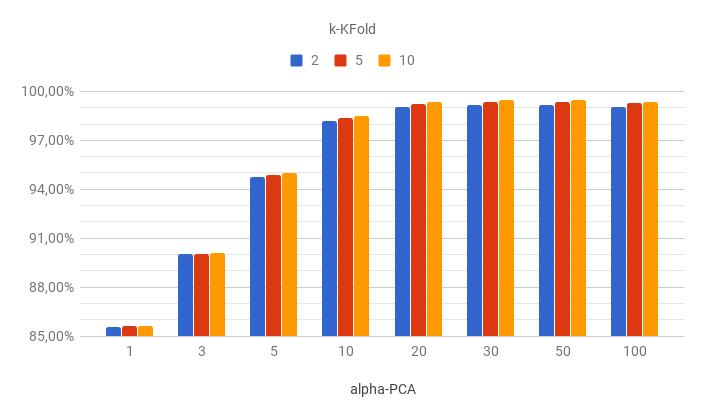
\includegraphics[width=\textwidth]{graficos/cv_cmp_folds_accuracy.png}
    \caption{Promedio de accuracy en función de alpha-PCA agrupado por k-KFold}
    \label{fig:cv_cmp_folds_accuracy}
\end{figure}

\begin{figure}[H]
    \centering
    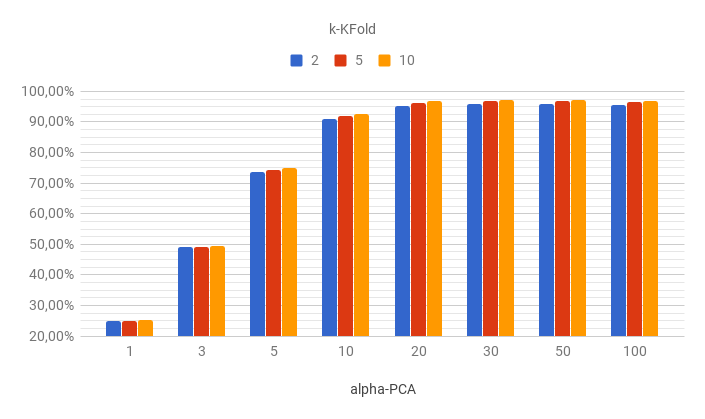
\includegraphics[width=\textwidth]{graficos/cv_cmp_folds_precision.png}
    \caption{Promedio de precision en función de alpha-PCA agrupado por k-KFold}
    \label{fig:cv_cmp_folds_precision}
\end{figure}

\begin{figure}[H]
    \centering
    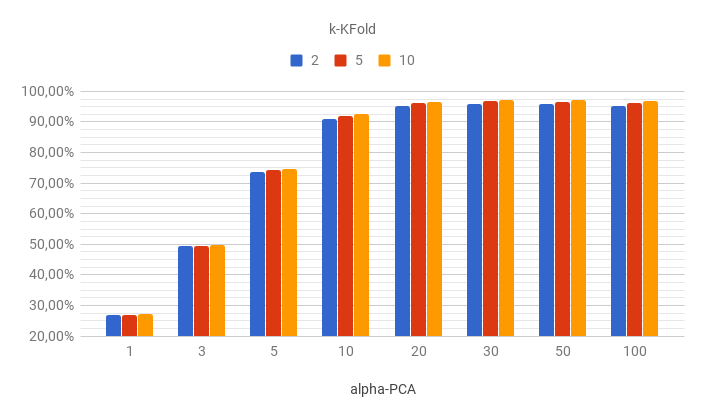
\includegraphics[width=\textwidth]{graficos/cv_cmp_folds_recall.png}
    \caption{Promedio de recall en función de alpha-PCA agrupado por k-KFold}
    \label{fig:cv_cmp_folds_recall}
\end{figure}

\subsubsection{Comparación de parámetros}

En cuanto al parámetro $\alpha$ se puede notar a primera vista en las figuras \ref{fig:cv1_accuracy}, \ref{fig:cv1_precision} y \ref{fig:cv1_recall} que, como se había planteado en la hipótesis, la calidad de los resultados crece junto con $\alpha$, pero existe un punto a partir del cual se estanca este crecimiento debido a que la información que aportan las componentes que se van agregando es muy poca. En este caso, dicho punto parece encontrarse alrededor de $\alpha = 20$. Se observa también que mejores resultados aparecen a partir de $\alpha = 10$.

\begin{figure}[H]
    \centering
    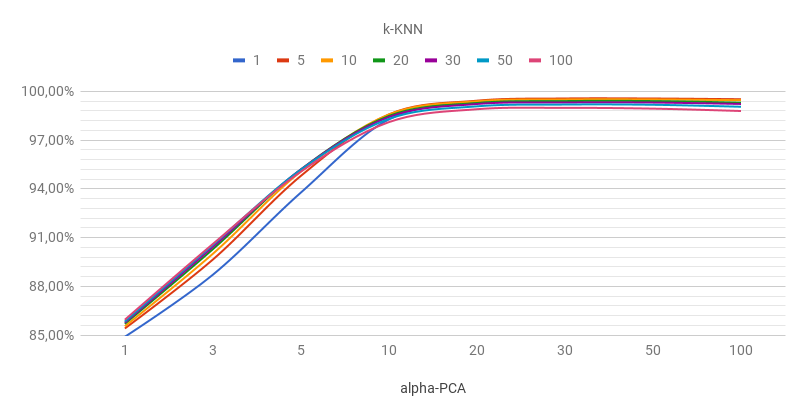
\includegraphics[width=\textwidth]{graficos/cv1_accuracy.png}
    \caption{Accuracy en función de alpha-PCA para cada k-KNN}
    \label{fig:cv1_accuracy}
\end{figure}

\begin{figure}[H]
    \centering
    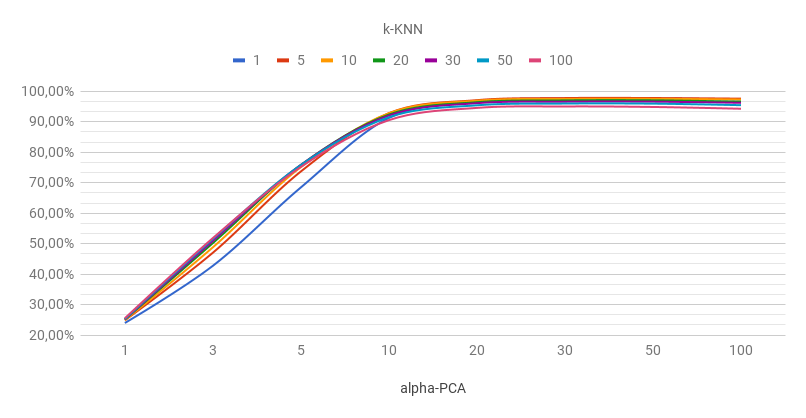
\includegraphics[width=\textwidth]{graficos/cv1_precision.png}
    \caption{Precision en función de alpha-PCA para cada k-KNN}
    \label{fig:cv1_precision}
\end{figure}

\begin{figure}[H]
    \centering
    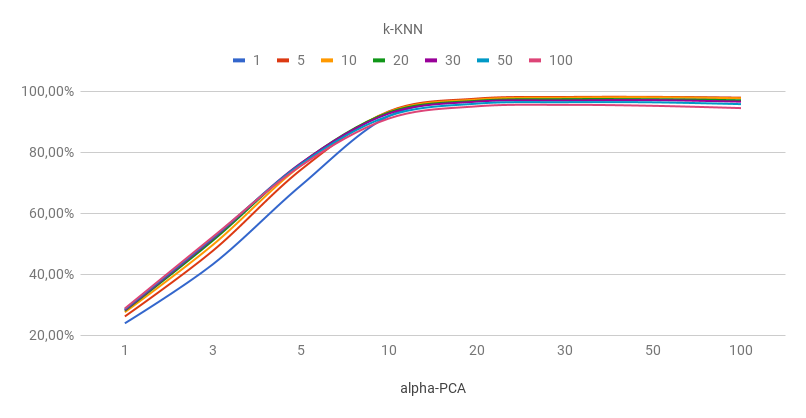
\includegraphics[width=\textwidth]{graficos/cv1_recall.png}
    \caption{Recall en función de alpha-PCA para cada k-KNN}
    \label{fig:cv1_recall}
\end{figure}

Mirando los gráficos más de cerca (figuras \ref{fig:cv1_accuracy_zoom}, \ref{fig:cv1_precision_zoom}, \ref{fig:cv1_recall_zoom}) se puede ver que los valores 1, 5 y 10 de k-KNN son los que tienen resultados superiores. Sorprendentemente, $k = 1$ es incluso mejor que $k = 10$. En la hipótesis se había mencionado que una imagen de una clase podía tener vecinos más cercanos de otra clase con similar escritura, por lo que valores muy pequeños de $k$ podrían seleccionar erróneamente a esta otra clase. Sin embargo, estos resultados sugieren que, para la base de entrenamiento usada, esta situación no se presenta muy frecuentemente.

Por otra parte, se ve claramente que luego de pasar el valor óptimo de $k$ la calidad de los resultados decrece a medida que aumenta la cantidad de vecinos considerados, como se esperaba.

Con respecto a $\alpha$ se observa que para los últimos valores medidos la calidad de los resultados empieza a decrecer, a diferencia de lo que se había dicho en la hipótesis. Una posible explicación que se pudo encontrar para este comportamiento considera el error inherente de la aritmética de números reales en una computadora:

El algoritmo de PCA obtiene de la matriz de covarianza los autovectores necesarios para determinar el cambio de base necesario. Para esto utiliza el método de la potencia, el cual realiza una serie de operaciones aritméticas de matrices por una cantidad determinada de iteraciones, introduciendo en cada iteración un error que se arrastra a las iteraciones siguientes. Luego de obtener cada autovector es necesario aplicar deflación para poder hallar el siguiente. En este procedimiento se utilizan este autovalor y autovector hallados. Esto implica que el cómputo de cada autovector arrastra los errores del cómputo de todos los autovectores anteriores. Luego, a medida que crece el valor de $\alpha$ este error se hace cada vez mayor, distorsionando cada vez más la información de las imágenes, lo que resulta en un decrecimiento de la calidad de los resultados.

\begin{figure}[H]
    \centering
    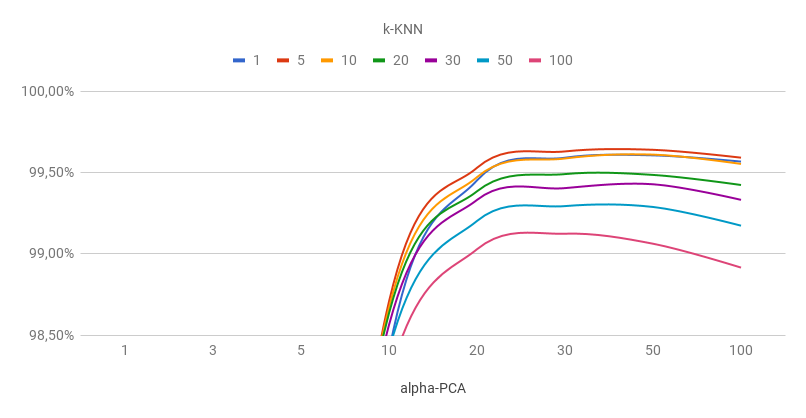
\includegraphics[width=\textwidth]{graficos/cv1_accuracy_zoom.png}
    \caption{Accuracy en función de alpha-PCA para cada k-KNN}
    \label{fig:cv1_accuracy_zoom}
\end{figure}

\begin{figure}[H]
    \centering
    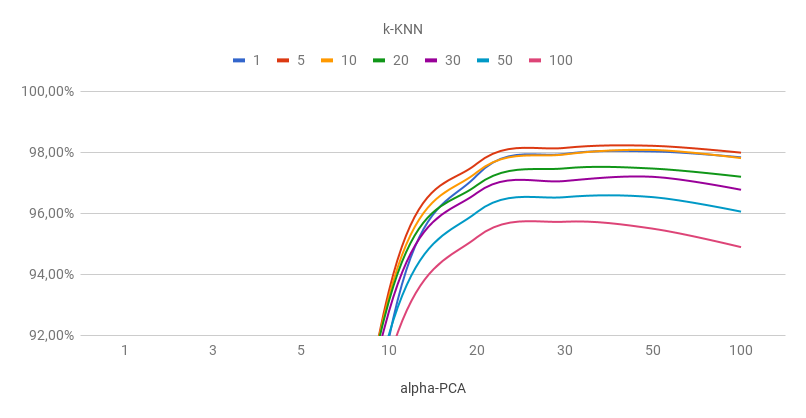
\includegraphics[width=\textwidth]{graficos/cv1_precision_zoom.png}
    \caption{Precision en función de alpha-PCA para cada k-KNN}
    \label{fig:cv1_precision_zoom}
\end{figure}

\begin{figure}[H]
    \centering
    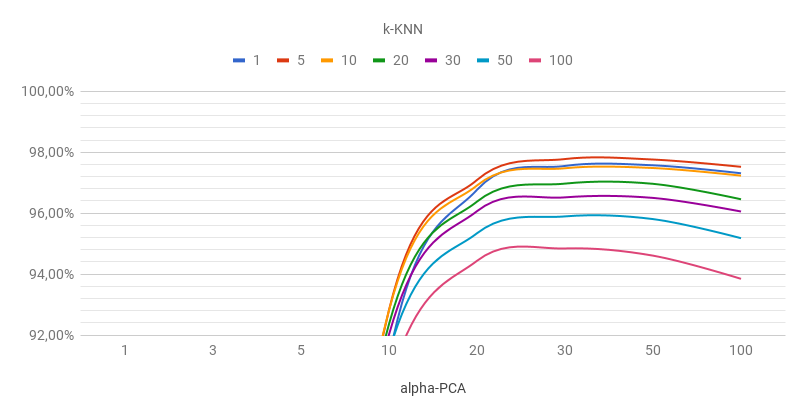
\includegraphics[width=\textwidth]{graficos/cv1_recall_zoom.png}
    \caption{Recall en función de alpha-PCA para cada k-KNN}
    \label{fig:cv1_recall_zoom}
\end{figure}

Con esta primera búsqueda se puede concluir entonces que los valores óptimos de alpha-PCA se encuentran entre 20 y 50, y los de k-KNN entre 1 y 10. Luego se realiza una segunda búsqueda más granular en estos rangos.

\subsection{Segunda búsqueda}

\subsection{Tomando mas rigurosidad}

\subsubsection{Resultados}


\subsubsection{Análisis de resultados}



\section{Variando tamaño del set de entrenamiento}

En esta parte probaremos distintos k para distintos tamaños de set de entrenamiento, para poder observar si se encuentra alguna diferencia entre los tamaños y su k en kNN.
Para poder ver esto, tomamos la misma cantidad de imágenes de cada clase aleatoriamente. Los tamaños elegidos fueron [5000, 10000, 20000, 30000, 42000], la variable $\alpha$ la mantuvimos como la optima que se obtuvo en el experimento anterior, el k se utilizo entre[1, 5, 10, 20, 50, 75, 100] y el K de K-fold lo mantuvimos en 5.

\subsection{Hipótesis}

Nuestra hipótesis sera que a medida que el tamaño del set de entrenamiento decrece y mientras el k crece, los resultados decrecerán estrepitamente. En primer lugar si el k crece, como fue demostrado en el experimento anterior, veremos disminuciones en la eficacia. En segundo lugar, mientras el set de entrenamiento se achica, se tendrán menos datos para entrenar y el algoritmo de kNN tomara muchos valores, lo cual terminara resultando en una mala predicción.

\subsection{Resultados}


\subsection{Análisis de los Resultados}

A partir de este resultado podemos reafirmar la hipótesis del experimento anterior y se pude decir que se cumplió con lo esperado, ya que al disminuir la cantidad de imágenes de entrenamiento, tanto el accuracy como el f1 score bajan. Tambien se observa que con con k muy altos, para el caso de 5000 imágenes, el porcentaje baja linealmente, lo cual cumple con lo que decíamos.